\chapter{Connecting and Breakout Board: Schematic and Measuring}\label{ConnectingBreakoutBoard} 
\textbf{Name: Group 630}\\
\textbf{Date: 15/04 - 2016}

\subsubsection{Purpose}
Schematic of the Connecting and Breakout Board and Measuring of the system.

%\subsubsection{Setup}
\begin{figure}[H]
  \centering
	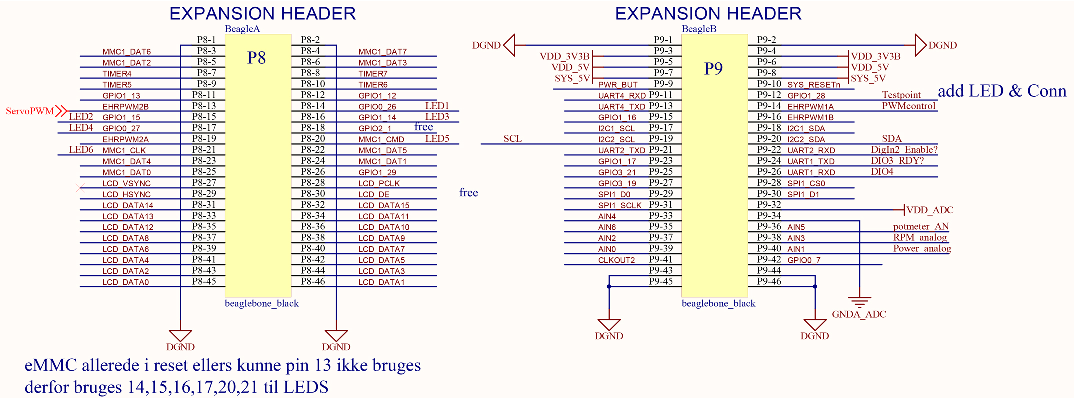
\includegraphics[scale=0.92]{figures/ExpanionHeader.pdf}
	\caption{Expansion header diagram}
	\label{labExpanionHeader}
\end{figure}\vspace{-5mm}


\begin{figure}[H]
	\centering
	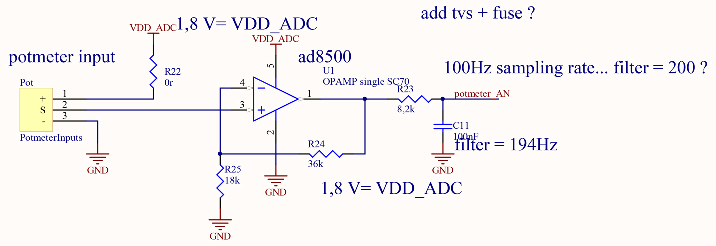
\includegraphics[scale=0.92]{figures/Potmeter.pdf}
	\caption{Potmeter diagram}
	\label{labPotmeter}
\end{figure}\vspace{-5mm}


\begin{figure}[H]
	\centering
	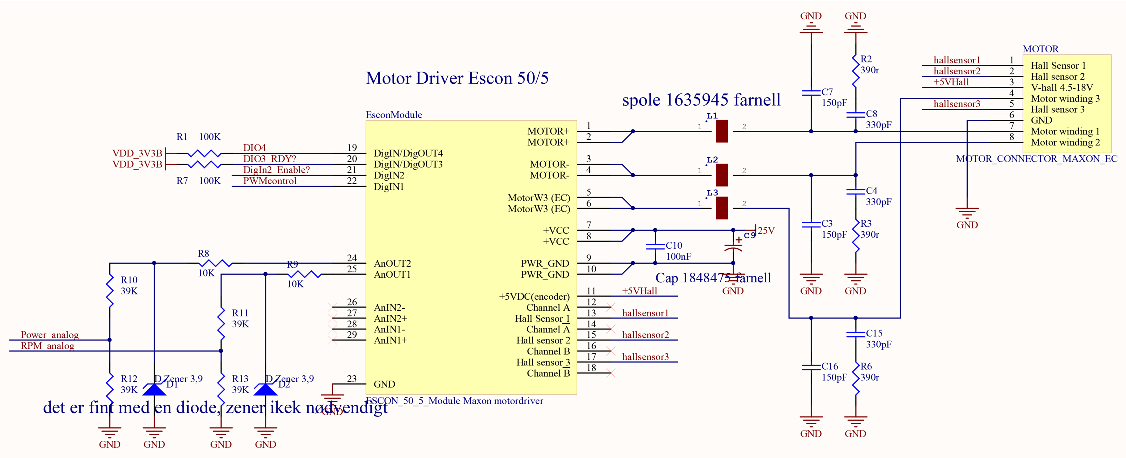
\includegraphics[scale=0.92]{figures/MotorDriver.pdf}
	\caption{Motor Driver diagram}
	\label{labMotorDriver}
\end{figure}\vspace{-5mm}


\begin{figure}[H]
	\centering
	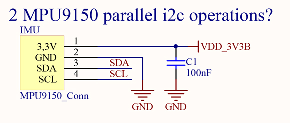
\includegraphics[scale=0.92]{figures/PMU9150.pdf}
	\caption{PMU9150 diagram}
	\label{labPMU9150}
\end{figure}\vspace{-5mm}


\begin{figure}[H]
	\centering
	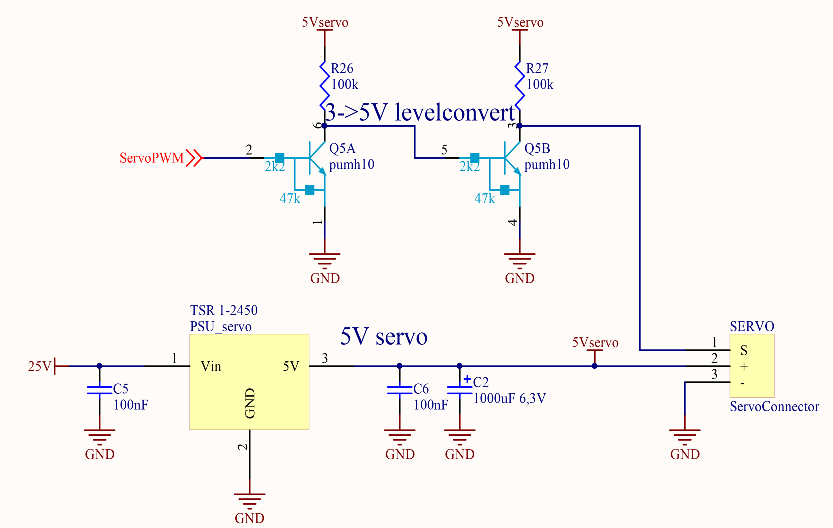
\includegraphics[scale=0.92]{figures/ServoMotor.pdf}
	\caption{Servo Motor diagram}
	\label{labServoMotor}
\end{figure}\vspace{-5mm}


\begin{figure}[H]
	\centering
	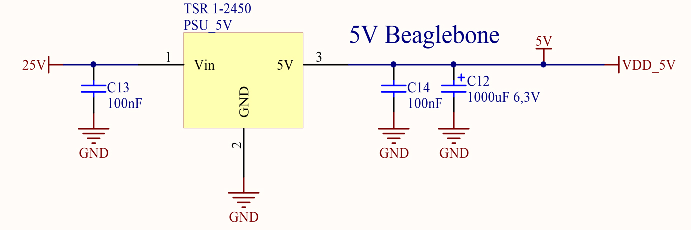
\includegraphics[scale=0.92]{figures/BeagleBone.pdf}
	\caption{Beagle Bone diagram}
	\label{labBeagleBone}
\end{figure}\vspace{-5mm}


\begin{figure}[H]
	\centering
	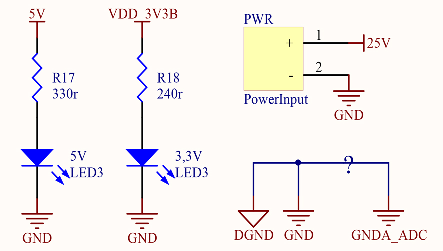
\includegraphics[scale=0.92]{figures/Power.pdf}
	\caption{Power diagram}
	\label{labPower}
\end{figure}\vspace{-5mm}


\begin{figure}[H]
	\centering
	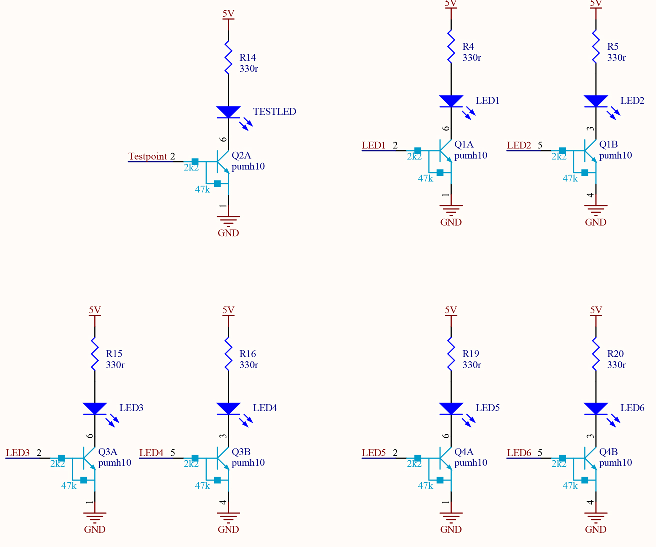
\includegraphics[scale=0.92]{figures/Led.pdf}
	\caption{LED diagram}
	\label{labLed}
\end{figure}\vspace{-5mm}


%
%\subsubsection{List of Equipment}
%\begin{table}[H]
%	\begin{tabular}{|l|l|p{4.3cm}|}
%		\hline%------------------------------------------------------------------------------------------------------------
%		\textbf{Instrument}                                  &  \textbf{AAU-no.}  &  \textbf{Type}                       \\
%		\hline%------------------------------------------------------------------------------------------------------------
%		Multimeter                                           &  60760           &  Fluke 189 Multimeter		                   \\
%		\hline%------------------------------------------------------------------------------------------------------------
%		Dedicated Power Supply of Cubli \small{(24 V - 3 A)} &  AAU3                   &  XP Power, AEB70US24                 \\
%		\hline%------------------------------------------------------------------------------------------------------------
%		Digital Protractor                                   &  None               & CMT Orange Tools     \\
%		\hline%------------------------------------------------------------------------------------------------------------
%	\end{tabular}
%\end{table}
%
%\subsubsection{Procedure}
%\begin{enumerate}
%  \item The Cubli base frame is leveled and the angle of equilibrium point is measured.
%  \item The frame is dismounted from the base frame and weight.
%  \item The frame is mounted back on the base frame after been rotated 90 degrees and the angle of equilibrium point is measured.
%  \item The Cubli frame is returned to original placement on the base frame.
%\end{enumerate}
%
%\subsubsection{Results}
%\begin{table}[H]
%	\begin{tabular}{|l|l|p{4.3cm}|}
%		\hline%------------------------------------------------------------------------------------------------------------
%		\textbf{Frame rotation angle in degrees}       &  \textbf{Angle form equilibrium point in degrees}         \\
%		\hline%------------------------------------------------------------------------------------------------------------
%		0                                & 2,50           \\
%		\hline%------------------------------------------------------------------------------------------------------------
%		90							  & 4,50              \\
%		\hline%------------------------------------------------------------------------------------------------------------
%	\end{tabular}
%\end{table}
%
%\subsubsection{Results}
%\begin{table}[H]
%	\begin{tabular}{|l|l|p{4.3cm}|}
%		\hline%------------------------------------------------------------------------------------------------------------
%		\textbf{Weight of the frame}       &  \textbf{Gram}         \\
%		\hline%------------------------------------------------------------------------------------------------------------
%		 Fully mounted frame        	  & 770          \\
%		\hline%------------------------------------------------------------------------------------------------------------
%	\end{tabular}
%\end{table}	
